\section{Phân tích khám phá dữ liệu (EDA)}

Phần này tổng hợp các nhận xét trực quan từ những biểu đồ EDA trong thư mục \texttt{img/}. Mục tiêu là nêu ra đặc điểm chính của dữ liệu trước khi huấn luyện mô hình phát hiện vi phạm không đội mũ bảo hiểm.

\subsection{Tổng quan Dataset}
Tập dữ liệu được chia thành 3 tập \texttt{train}, \texttt{val}, \texttt{test}. Bảng sau mô tả số lượng ảnh và nhãn theo từng split:
\begin{table}[H]
\centering
\caption{Tổng quan số lượng ảnh và annotations theo split}
\begin{tabular}{lrrr}
\toprule
Split & Số ảnh & Số annotations & Avg ann/ảnh \\
\midrule
train & 2309 & 6965 & 3.02 \\
val   & 330  & 1889 & 5.72 \\
test  & 659  & 1861 & 2.82 \\
\midrule
\textbf{TOTAL} & \textbf{3298} & \textbf{10715} & \textbf{3.25} \\
\bottomrule
\end{tabular}
\end{table}

\noindent Nhìn chung, tập dữ liệu có quy mô đủ lớn để huấn luyện, tuy nhiên mật độ nhãn trên mỗi ảnh không đồng đều giữa các split.

\subsection{Phân bố thuộc tính bounding box}
\begin{figure}[H]
    \centering
    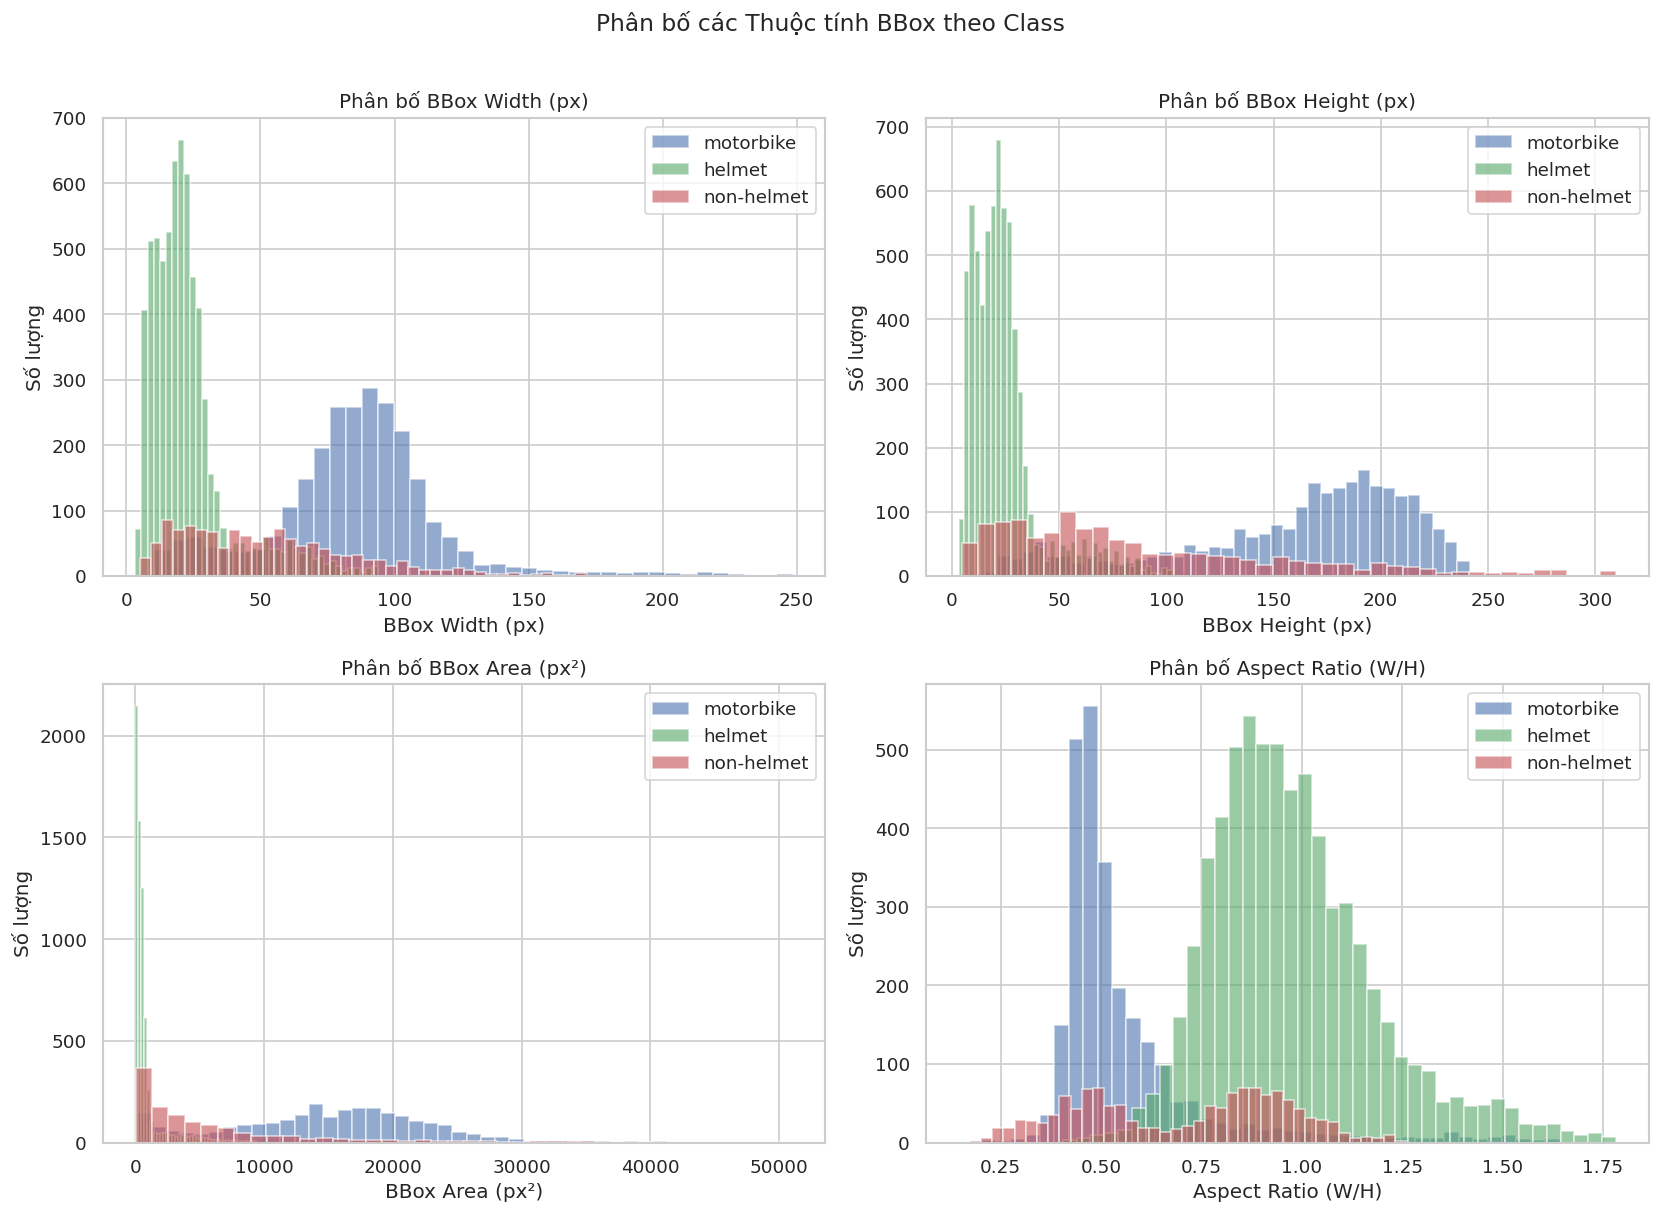
\includegraphics[width=0.95\textwidth]{img/bbox_distributions.png}
    \caption{Phân bố Width, Height, Area và Aspect Ratio của bounding box}
\end{figure}

Biểu đồ cho thấy phần lớn bounding box tập trung ở kích thước nhỏ đến trung bình; đuôi phân bố kéo dài về phía kích thước lớn cho thấy vẫn tồn tại một số đối tượng rất lớn trong khung hình. Tỷ lệ khung hình tập trung quanh một vài vùng đặc trưng, phản ánh sự khác biệt hình học giữa các lớp đối tượng.

\subsection{Phân bố nhãn và mật độ đối tượng theo ảnh}
\begin{figure}[H]
    \centering
    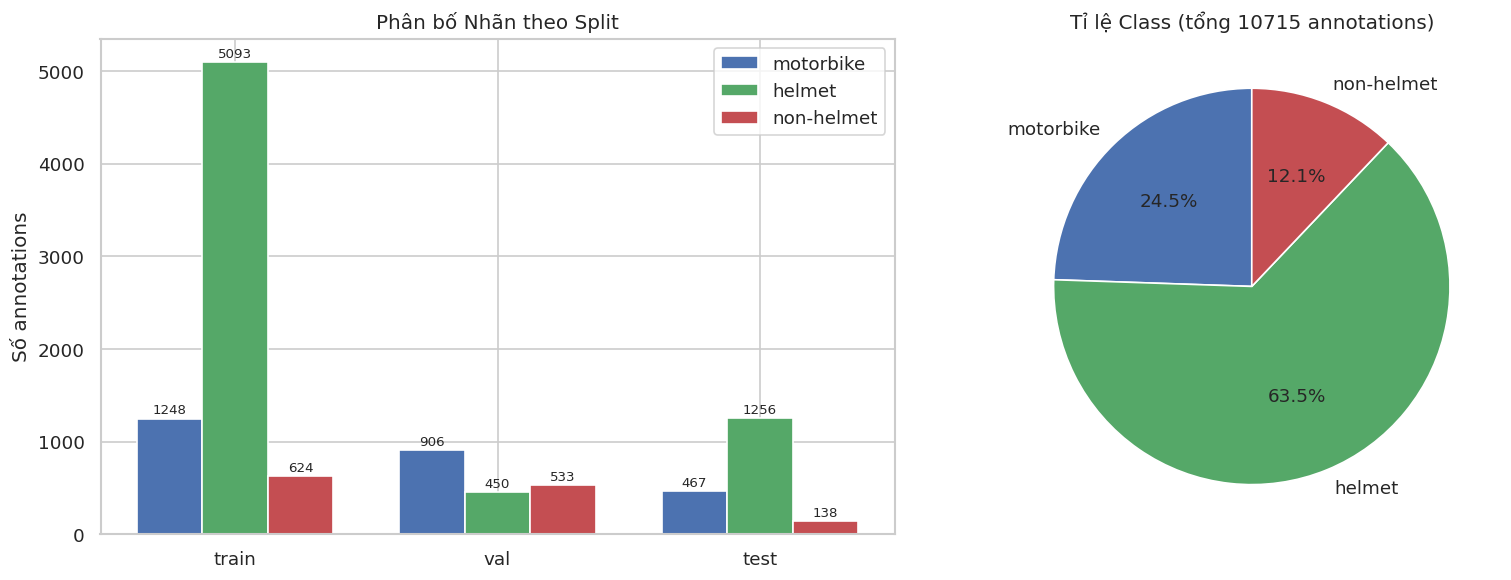
\includegraphics[width=0.85\textwidth]{img/class_distribution.png}
    \caption{Phân bố số lượng annotations theo từng lớp}
\end{figure}

\begin{figure}[H]
    \centering
    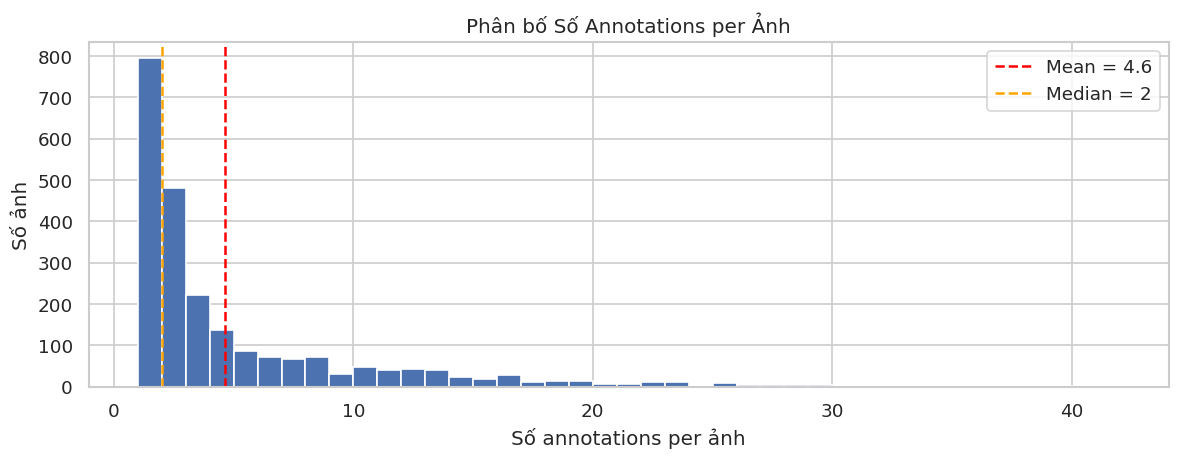
\includegraphics[width=0.85\textwidth]{img/ann_per_image.png}
    \caption{Phân bố số lượng annotations trên mỗi ảnh}
\end{figure}

Từ hai biểu đồ có thể rút ra:
\begin{itemize}
    \item Dữ liệu bị lệch lớp, trong đó lớp \texttt{non-helmet} là lớp thiểu số.
    \item Số lượng annotation trên mỗi ảnh phân bố không đều; phần lớn ảnh có ít đối tượng, trong khi một số ảnh chứa mật độ đối tượng cao.
\end{itemize}

\noindent Điều này có thể làm mô hình thiên lệch về lớp phổ biến và giảm khả năng phát hiện đúng lớp vi phạm nếu không có kỹ thuật cân bằng phù hợp.

\subsection{Quan hệ giữa các thuộc tính hình học}
\begin{figure}[H]
    \centering
    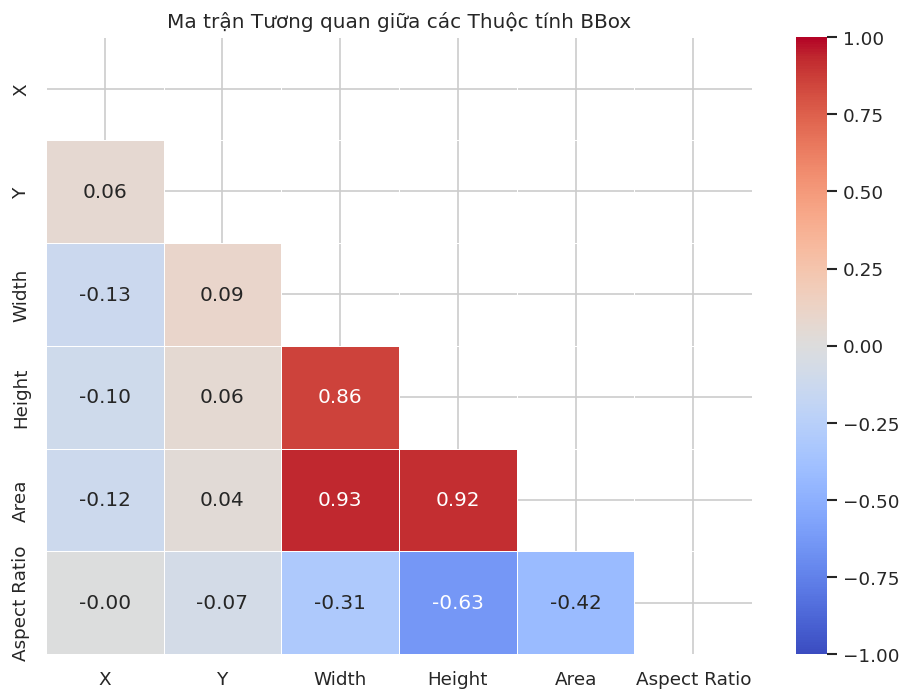
\includegraphics[width=0.85\textwidth]{img/correlation_matrix.png}
    \caption{Ma trận tương quan giữa các thuộc tính}
\end{figure}

\begin{figure}[H]
    \centering
    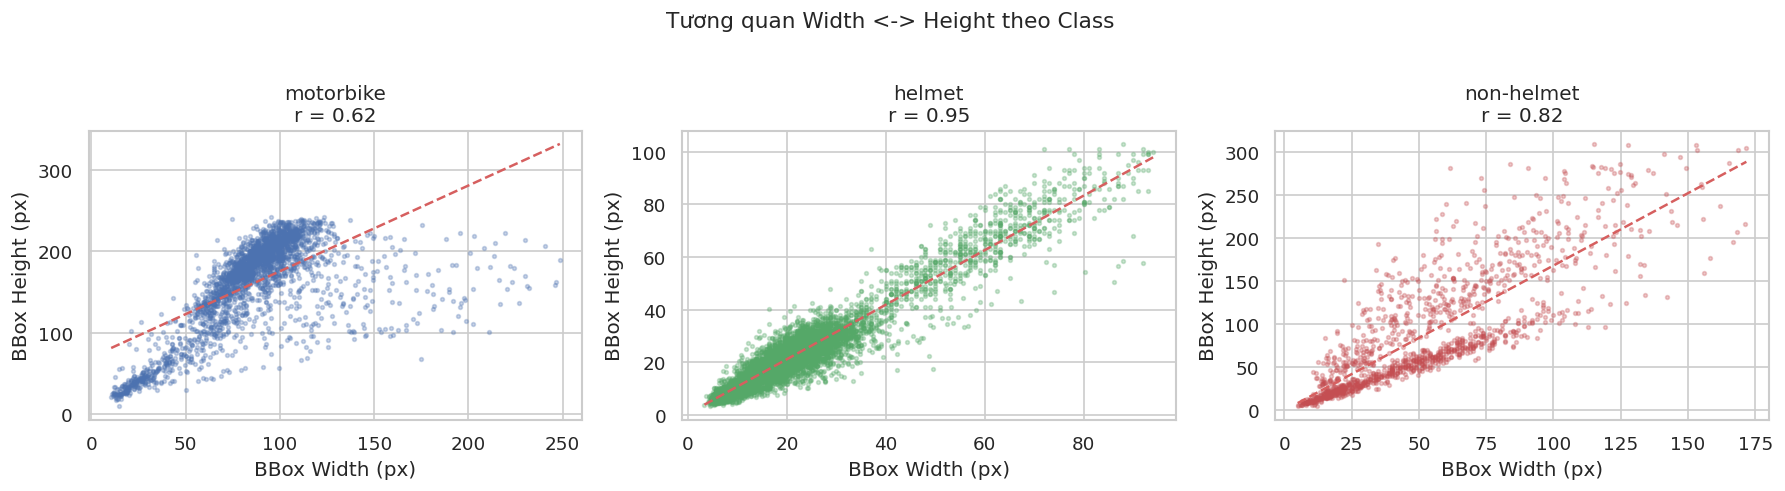
\includegraphics[width=0.9\textwidth]{img/width_height_scatter.png}
    \caption{Mối quan hệ giữa Width và Height theo lớp}
\end{figure}

\begin{figure}[H]
    \centering
    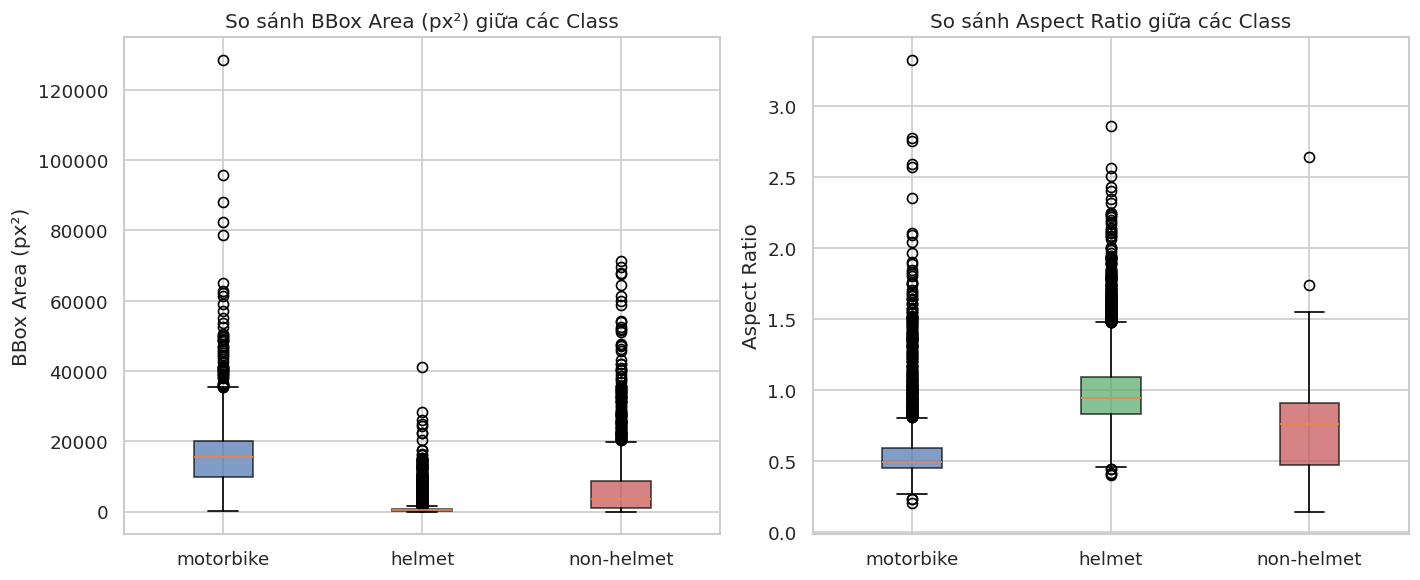
\includegraphics[width=0.85\textwidth]{img/class_comparison_boxplot.png}
    \caption{So sánh phân bố kích thước bounding box giữa các lớp}
\end{figure}

Các biểu đồ cho thấy chiều rộng và chiều cao có tương quan dương rõ rệt. Boxplot theo lớp cũng cho thấy khác biệt kích thước giữa các nhóm đối tượng: lớp \texttt{motorbike} thường có hộp lớn hơn, trong khi \texttt{helmet} và \texttt{non-helmet} nhỏ hơn và phân tán hẹp hơn.

\subsection{Phân bố vị trí đối tượng trong ảnh}
\begin{figure}[H]
    \centering
    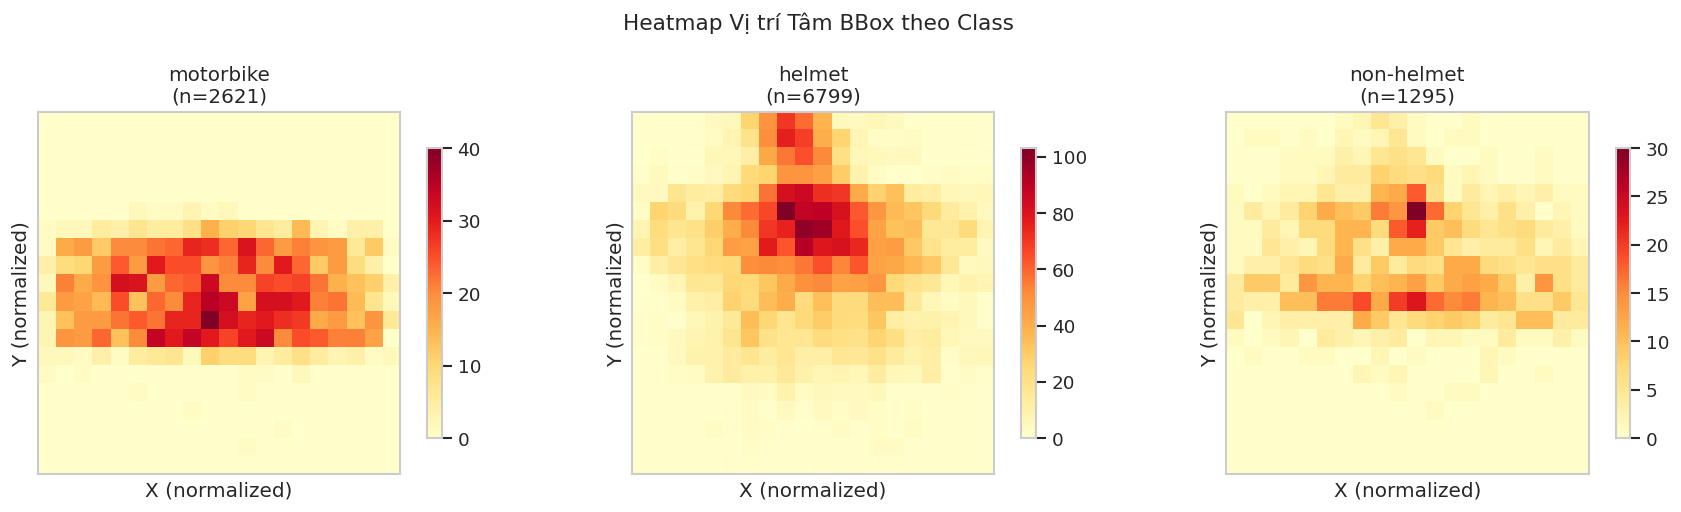
\includegraphics[width=0.85\textwidth]{img/bbox_heatmap.png}
    \caption{Heatmap vị trí trung tâm bounding box}
\end{figure}

Heatmap thể hiện tâm của bounding box tập trung nhiều ở vùng giữa ảnh, giảm dần về các vùng rìa. Điều này cho thấy dữ liệu mang thiên hướng bố cục trung tâm, mô hình có thể học tốt vùng trung tâm nhưng cần tăng cường dữ liệu để cải thiện khả năng tổng quát ở vùng biên.

\subsection{Đa dạng kích thước đối tượng}
\begin{figure}[H]
    \centering
    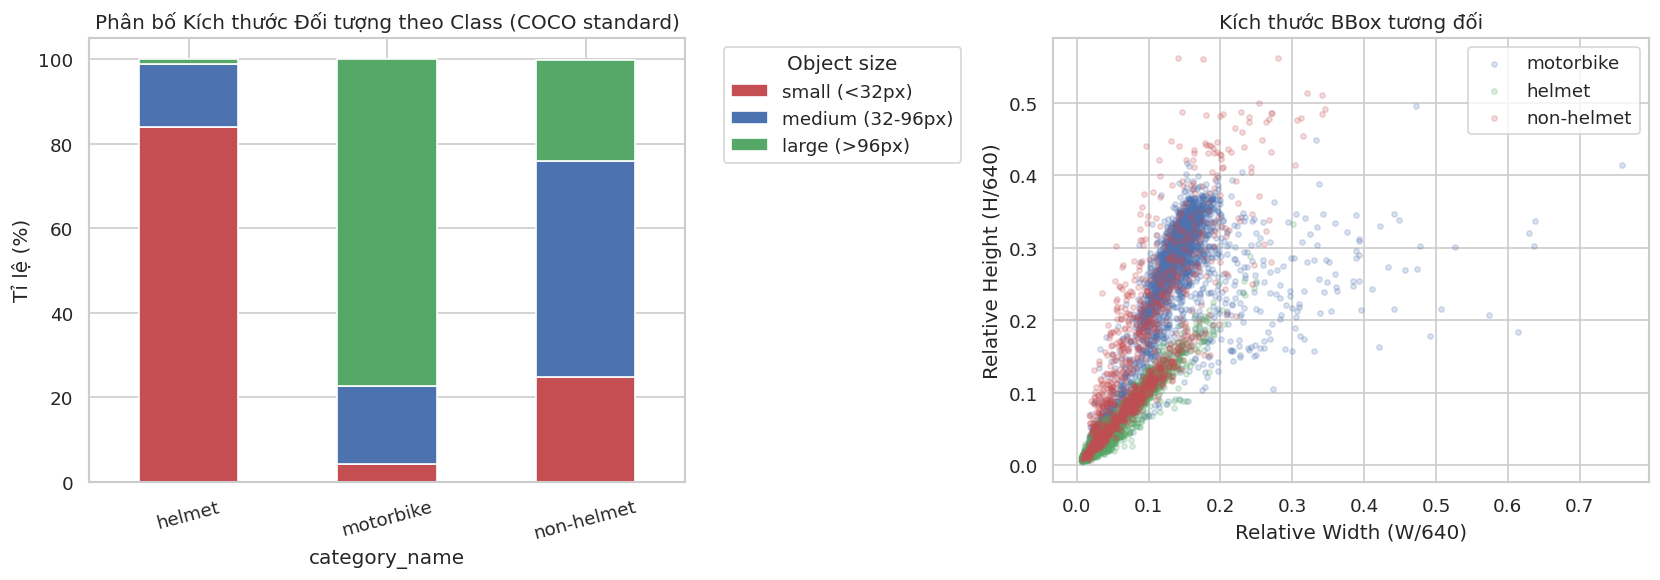
\includegraphics[width=0.85\textwidth]{img/object_size_diversity.png}
    \caption{Đa dạng kích thước đối tượng}
\end{figure}

Biểu đồ xác nhận dữ liệu chứa đồng thời small, medium, large objects, nhưng tỷ trọng nhóm nhỏ là đáng kể ở các lớp liên quan đến đầu người. Đây là đặc trưng quan trọng vì bài toán phát hiện vật thể nhỏ thường khó hơn và nhạy với độ phân giải đặc trưng.

\subsection{Chất lượng ảnh đầu vào}
\begin{figure}[H]
    \centering
    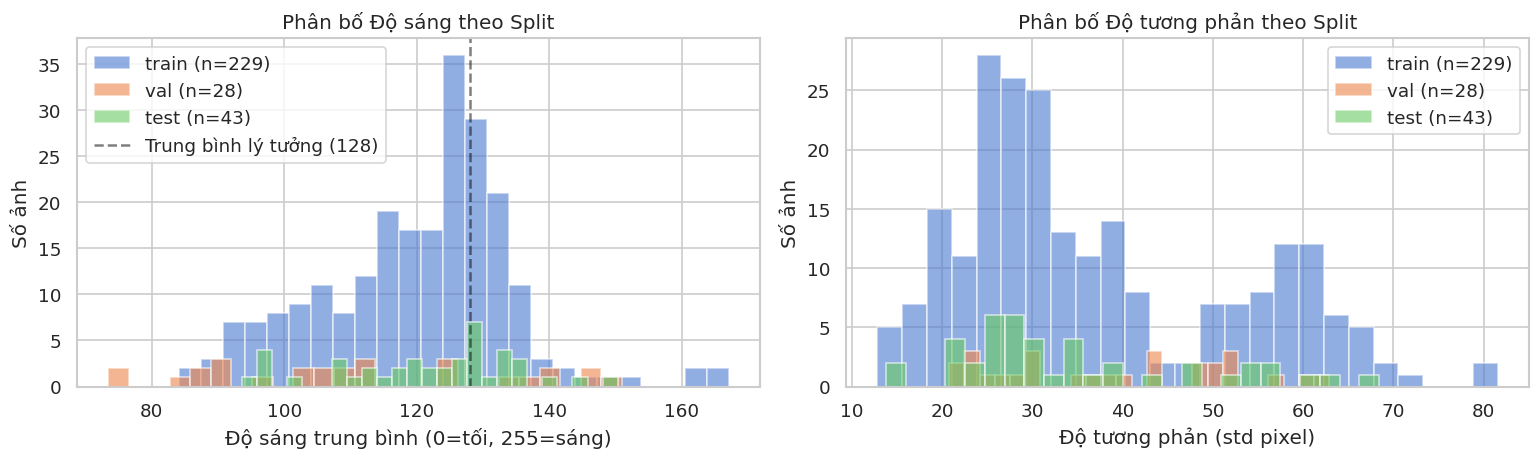
\includegraphics[width=0.9\textwidth]{img/brightness_contrast.png}
    \caption{Phân bố độ sáng và độ tương phản của dataset}
\end{figure}

\begin{figure}[H]
    \centering
    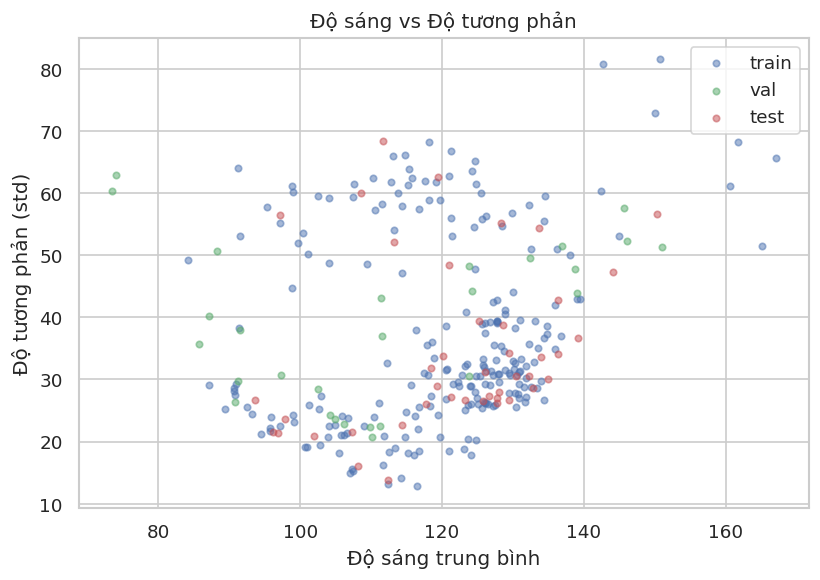
\includegraphics[width=0.85\textwidth]{img/brightness_contrast_scatter.png}
    \caption{Mối quan hệ giữa Brightness và Contrast}
\end{figure}

\begin{figure}[H]
    \centering
    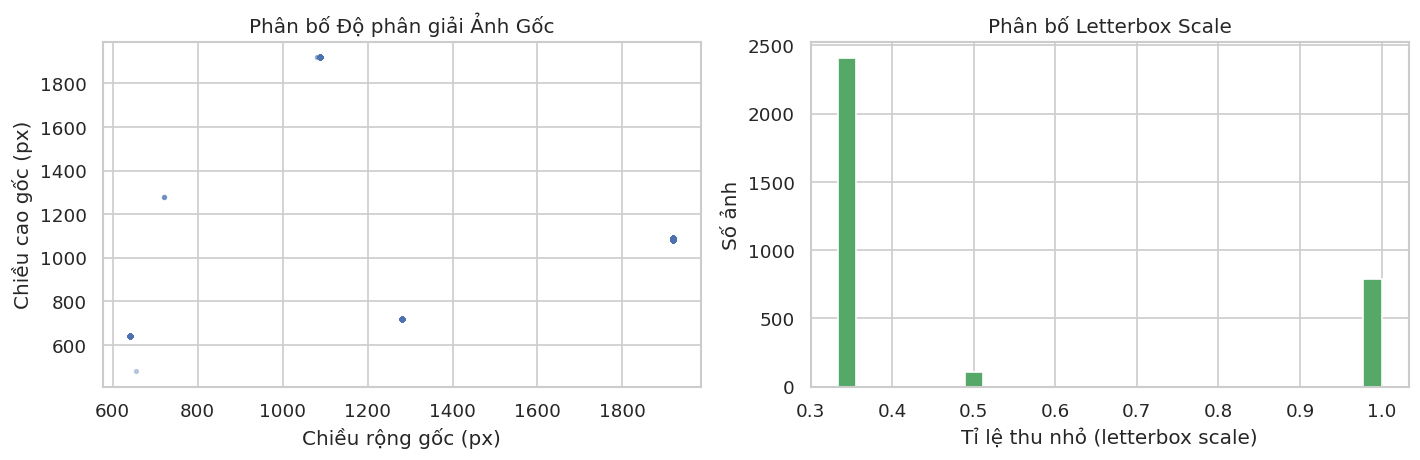
\includegraphics[width=0.85\textwidth]{img/resolution_letterbox.png}
    \caption{Kích thước ảnh sau resize (640$\times$640)}
\end{figure}

Phân bố brightness/contrast cho thấy dữ liệu bao phủ nhiều điều kiện chiếu sáng và mức tương phản khác nhau. Việc chuẩn hóa về kích thước đầu vào giúp ổn định pipeline huấn luyện, nhưng vẫn cần augmentation quang học để mô hình bền vững hơn trong bối cảnh thực tế.

\subsection{Mẫu ảnh trực quan}
\begin{figure}[H]
    \centering
    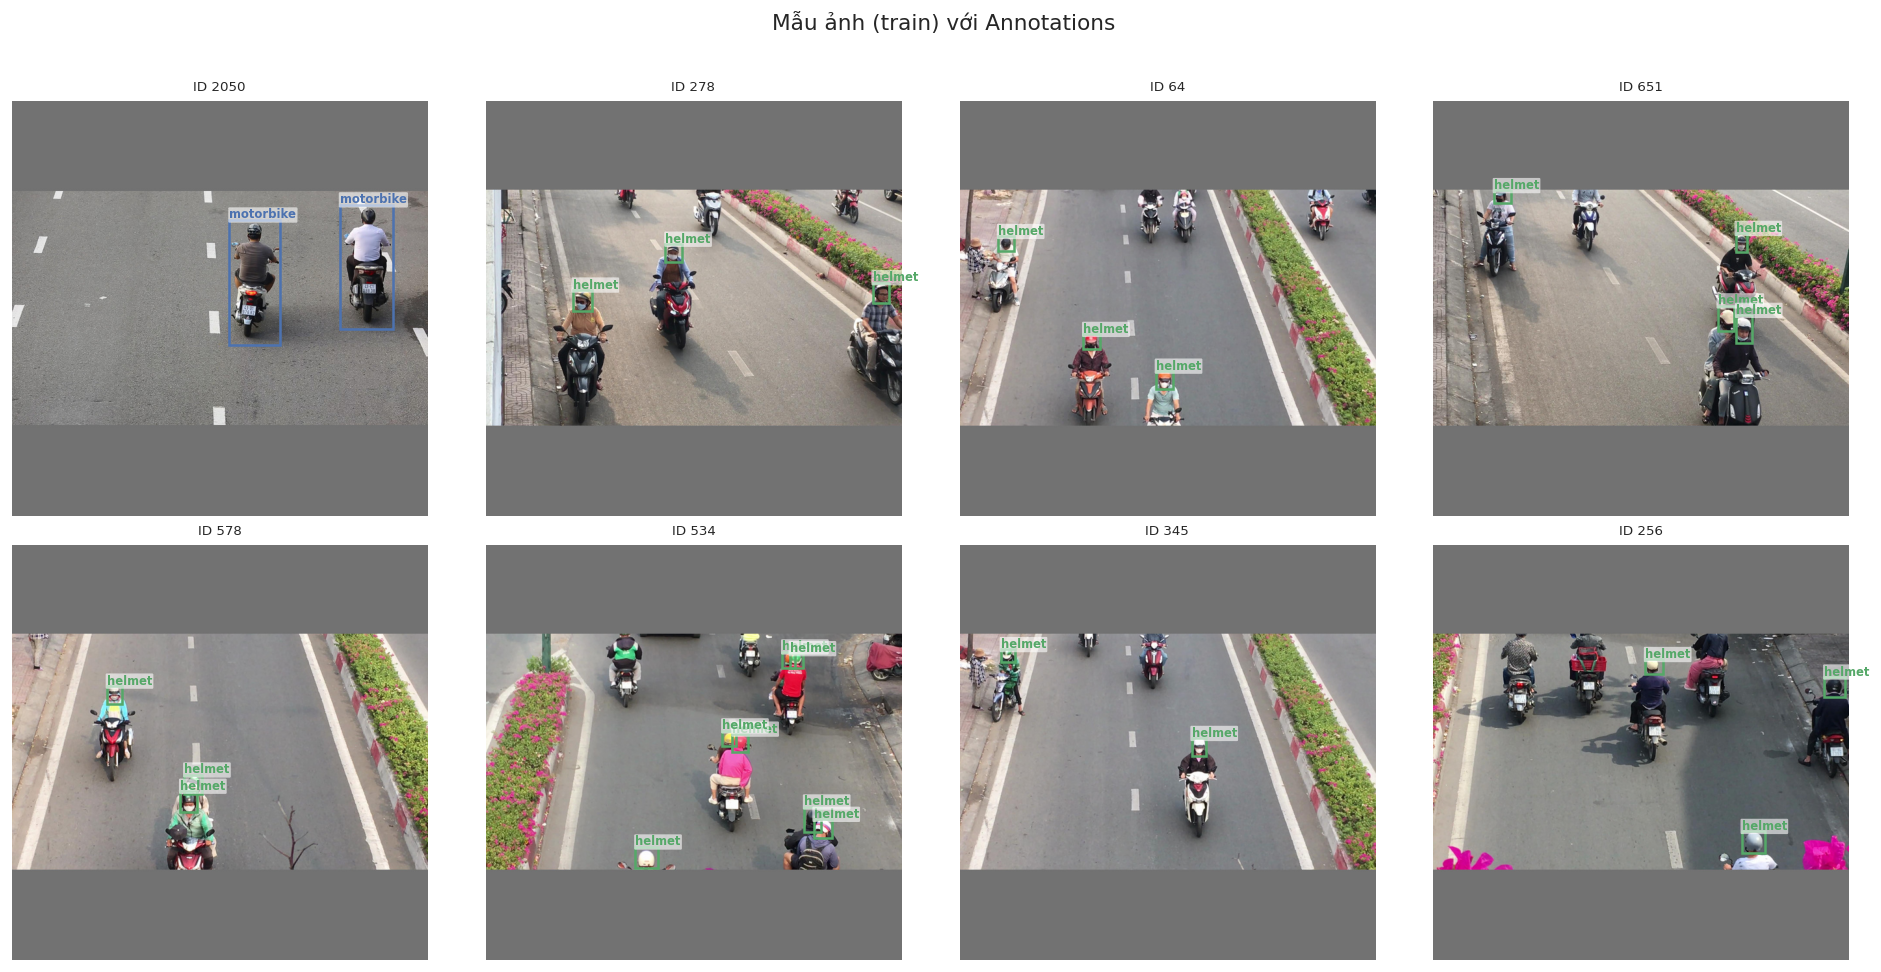
\includegraphics[width=0.95\textwidth]{img/samples_train.png}
    \caption{Mẫu ảnh từ tập train với bounding box}
\end{figure}

\begin{figure}[H]
    \centering
    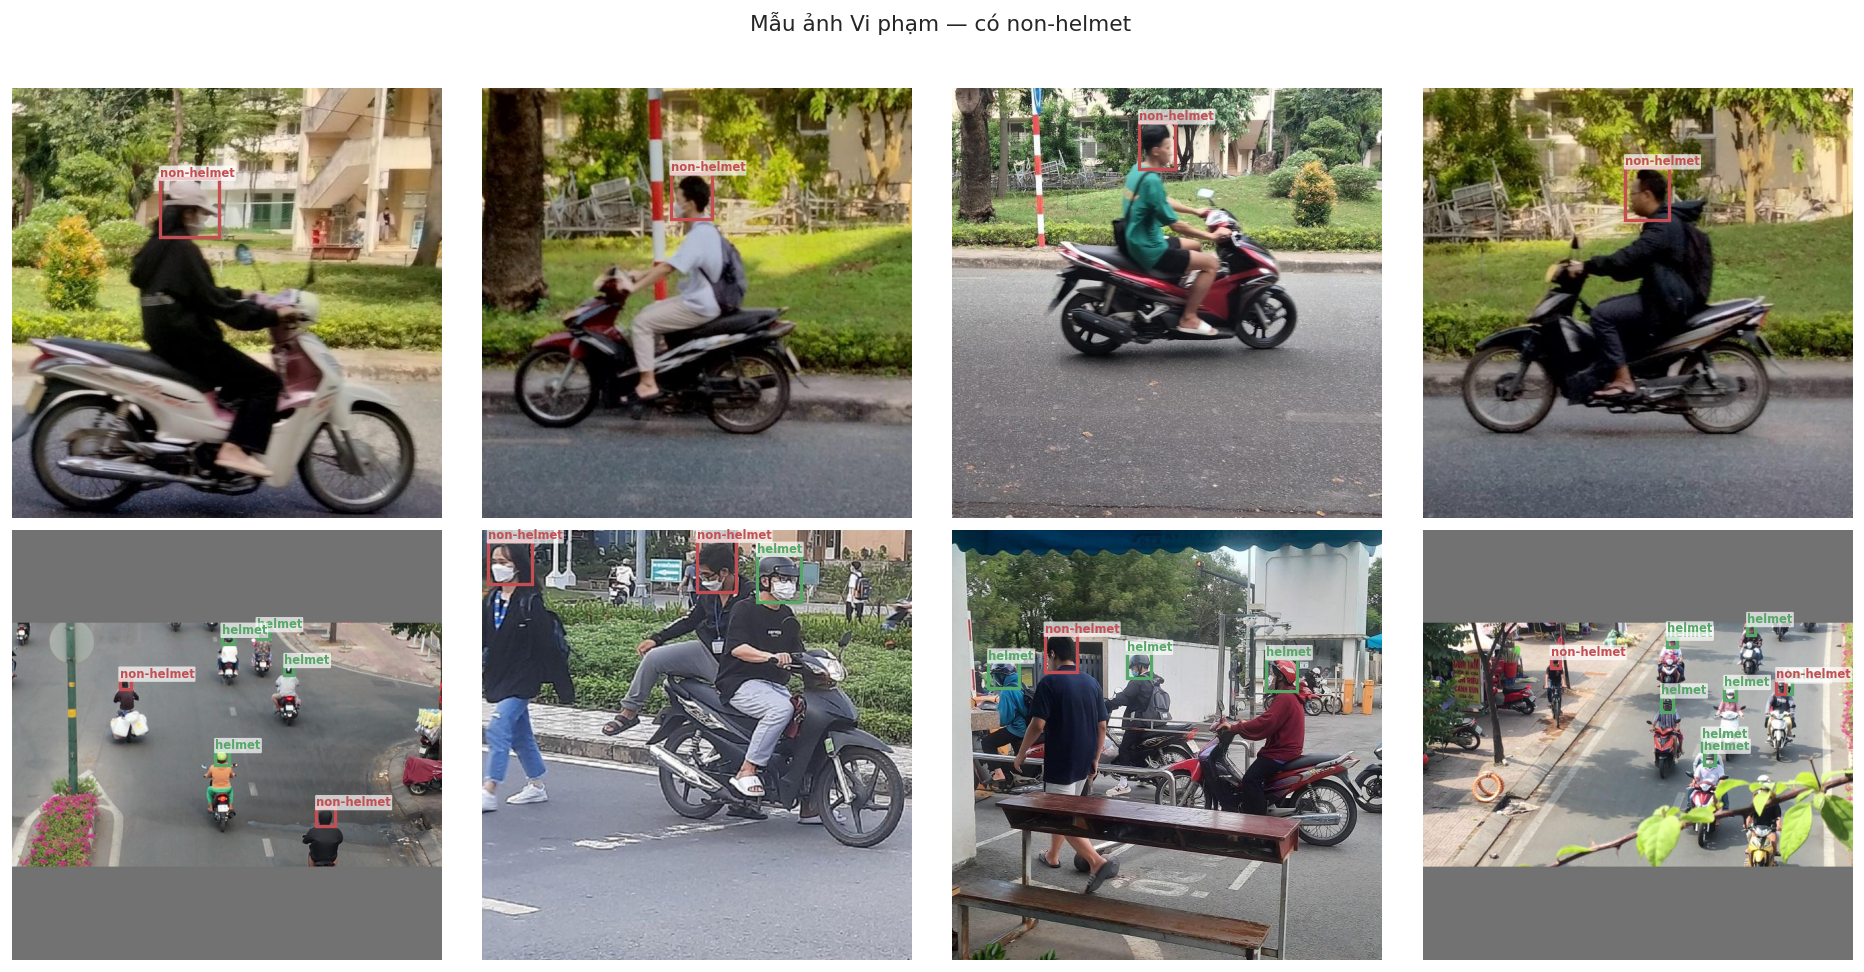
\includegraphics[width=0.95\textwidth]{img/samples_violation.png}
    \caption{Mẫu ảnh vi phạm (có non-helmet)}
\end{figure}

Các mẫu ảnh xác nhận dữ liệu có độ đa dạng về góc nhìn, bối cảnh giao thông và mức che khuất. Nhiều trường hợp vi phạm xuất hiện với kích thước nhỏ hoặc bị nhiễu nền, gây khó khăn trực tiếp cho mô hình.

\subsection{Tổng kết EDA}
\begin{itemize}
    \item Dataset có quy mô đủ để huấn luyện nhưng tồn tại mất cân bằng lớp, đặc biệt ở lớp vi phạm \texttt{non-helmet}.
    \item Đối tượng nhỏ chiếm tỷ lệ đáng kể, là thách thức chính của bài toán phát hiện.
    \item Vị trí đối tượng tập trung nhiều ở trung tâm ảnh, gợi ý cần tăng cường dữ liệu theo dịch chuyển không gian.
    \item Chất lượng ảnh khá đa dạng về ánh sáng và tương phản, phù hợp cho huấn luyện nếu kết hợp augmentation hợp lý.
\end{itemize}

Tóm lại, các biểu đồ EDA cho thấy bộ dữ liệu có nền tảng tốt, nhưng cần chiến lược huấn luyện hướng vào xử lý mất cân bằng lớp và cải thiện khả năng phát hiện vật thể nhỏ.
